\chapter{主成分分析 (PCA)}

本章将介绍主成分分析 (Principal Components Analysis, PCA) 方法,该方法旨在识别数据大致所在的子空间。PCA 的计算效率很高:它只需要进行特征向量计算(在 Matlab 中使用 \texttt{eig} 函数即可轻松完成)。

假设给定一个包含 $n$ 种不同类型汽车属性的数据集 $\{x^{(i)}; i = 1, \dots, n\}$,属性可能是最大速度、转弯半径等。令每个 $x^{(i)} \in \mathbb{R}^d$(其中 $d \ll n$)。但我们不知道的是,其中两个不同的属性——某个 $x_i$ 和 $x_j$——分别给出汽车的以英里/小时为单位的最大速度和以公里/小时为单位的最大速度。因此,这两个属性几乎呈线性相关,仅存在由于四舍五入到最接近的英里/小时或公里/小时而引入的微小差异。因此,数据实际上近似位于一个 $n-1$ 维子空间中。该如何自动检测并消除这种冗余?

举一个不那么牵强的例子,考虑一个对遥控直升机飞行员进行调查得到的数据集,其中 $x_1^{(i)}$ 是飞行员 $i$ 的飞行技能度量,而 $x_2^{(i)}$ 衡量他/她对飞行的喜爱程度。由于遥控直升机非常难飞,只有最投入、真正喜欢飞行的学生才能成为优秀的飞行员。因此,属性 $x_1$ 和 $x_2$ 强相关。事实上,我们可以假设数据实际上大致沿着某个对角线轴(即 $u_1$ 方向,捕捉了个人内在的飞行“天赋”)分布,只有少量噪声偏离该轴。(见下图。)我们如何自动计算这个 $u_1$ 方向?

\begin{figure}[H]
    \centering
    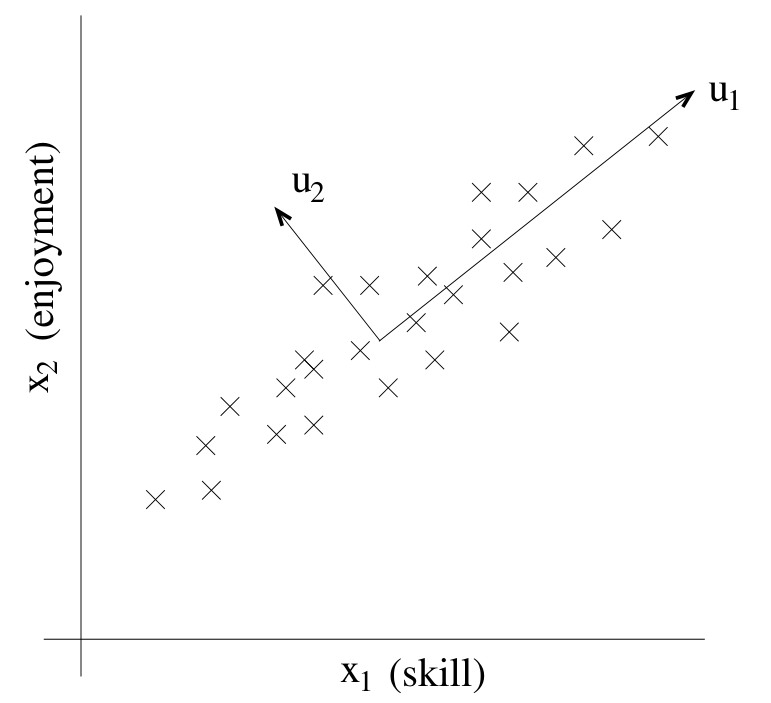
\includegraphics[width=0.6\textwidth]{figs/PCA.png}
\end{figure}

接下来将介绍 PCA 算法。但在正式运行 PCA 之前,通常首先通过归一化每个特征来预处理数据,使其均值为 0,方差为 1。具体做法是减去均值并除以经验标准差:
\[
    x_j^{(i)} \leftarrow \frac{x_j^{(i)} - \mu_j}{\sigma_j}
\]
其中 $\mu_j = \frac{1}{n} \sum_{i=1}^n x_j^{(i)}$ 和 $\sigma_j^2 = \frac{1}{n} \sum_{i=1}^n (x_j^{(i)} - \mu_j)^2$ 分别是特征 $j$ 的均值和方差。

减去 $\mu_j$ 会使均值变为零,对于已知均值为零的数据(例如,对应于语音或其他声学信号的时间序列)可以省略这一步。除以标准差 $\sigma_j$ 会将每个坐标重新缩放,使其具有单位方差,这确保了不同属性被视为同一“尺度”上的数据。例如,如果 $x_1$ 是汽车的最大速度(取值在几十到几百之间),而 $x_2$ 是座位数量(取值在 2-4 之间),那么这种重新归一化会重新缩放不同的属性,使它们更具可比性。如果已知不同属性都在同一尺度上,则可以省略这种缩放。一个例子是,如果每个数据点代表一个灰度图像,并且每个 $x_j^{(i)}$ 取值在 $\{0, 1, \dots, 255\}$ 之间,对应于图像 $i$ 中像素 $j$ 的强度值。

现在,数据已经归一化,如何计算“主要变化轴” $u$,即数据近似所在的那个方向?一种方法是将这个问题视为寻找单位向量 $u$,使得当数据被投影到对应于 $u$ 的方向上时,投影数据的方差最大化。直观地说,数据本身具有一定的方差/信息量。我们希望选择一个方向 $u$,使得如果我们将数据近似为位于对应于 $u$ 的方向/子空间中,则尽可能多地保留这些方差。

考虑以下已经归一化的数据集:

\begin{figure}[H]
    \centering
    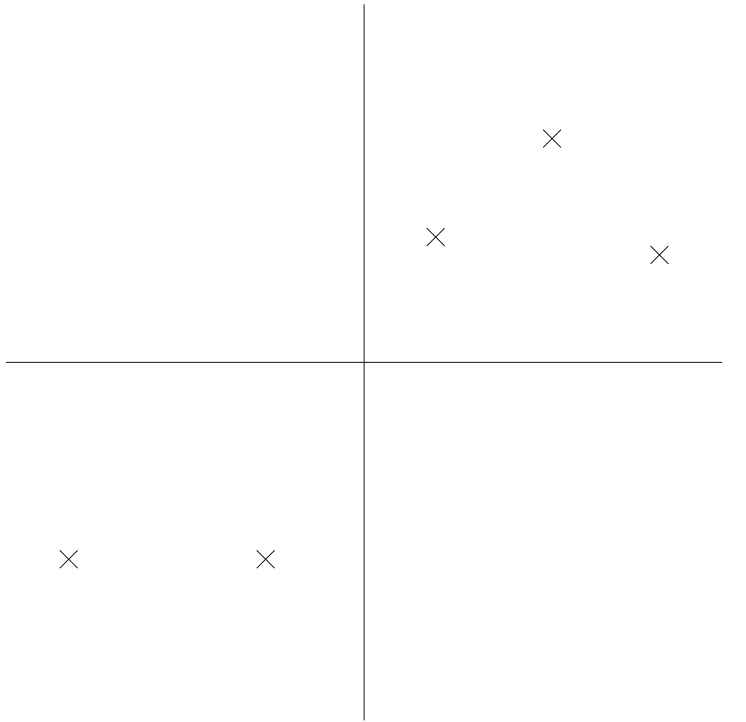
\includegraphics[width=0.6\textwidth]{figs/PCA_dataset.png}
\end{figure}

现在,假设选择的 $u$ 对应于下图所示的方向。圆圈表示原始数据点在该直线上的投影。

\begin{figure}[H]
    \centering
    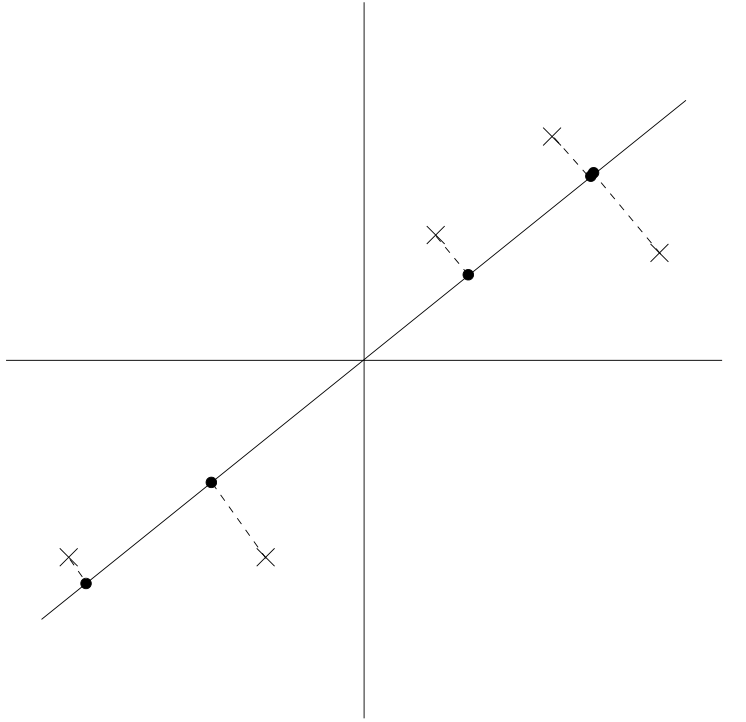
\includegraphics[width=0.6\textwidth]{figs/PCA_step1.png}
\end{figure}

可以看到,投影后的数据仍然具有相当大的方差,并且数据点倾向于远离零点。相比之下,如果选择以下方向:

\begin{figure}[H]
    \centering
    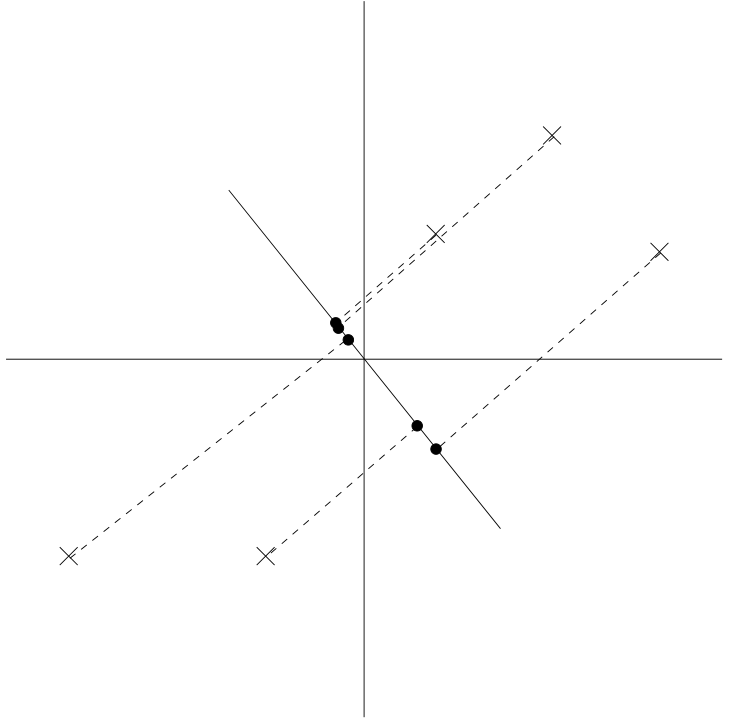
\includegraphics[width=0.6\textwidth]{figs/PCA_step2.png}
\end{figure}

在此方向上,投影的方差显著减小,并且更接近原点。

我们希望能够自动选择对应于上面所示两个图中的第一个图的方向 $u$。为了形式化这一点,请注意,给定一个单位向量 $u$ 和一个点 $x$, $x$ 在 $u$ 上的投影长度由 $x^T u$ 给出。也就是说,如果 $x^{(i)}$ 是数据集中的一个点(图中交叉点之一),那么它在 $u$ 上的投影(图中对应的圆圈)到原点的距离为 $x^{(i)T} u$。因此,为了最大化投影的方差,需要选择一个单位长度向量 $u$ 来最大化:
\begin{align*}
    \frac{1}{n} \sum_{i=1}^n (x^{(i)T} u)^2 
    &= \frac{1}{n} \sum_{i=1}^n u^T x^{(i)} x^{(i)T} u \\
    &= u^T \left( \frac{1}{n} \sum_{i=1}^n x^{(i)} x^{(i)T} \right) u.
\end{align*}
容易看出,在约束 $\|u\|_2 = 1$ 下最大化这个表达式会得到 $\Sigma = \frac{1}{n} \sum_{i=1}^n x^{(i)} x^{(i)T}$ 的主特征向量,这正是数据的经验协方差矩阵(假设数据均值为零)。\footnote{可以尝试使用拉格朗日乘子法来最大化 $u^T \Sigma u$,约束条件为 $u^T u = 1$。能够证明 $\Sigma u = \lambda u$ 对于某个 $\lambda$ 成立,这意味着 $u$ 是 $\Sigma$ 的特征向量,$\lambda$ 是对应的特征值。}

总而言之,如果希望找到一个一维子空间来近似数据,应该选择 $u$ 作为 $\Sigma$ 的主特征向量。更一般地,如果希望将数据投影到 $k$ 维子空间($k < d$),应该选择 $u_1, \dots, u_k$ 作为 $\Sigma$ 的前 $k$ 个特征向量。这些 $u_i$ 现在构成数据的一组新的正交基。\footnote{由于 $\Sigma$ 是对称的,所以 $u_i$ 是(或总是可以选择是)彼此正交的。}

然后,为了在该基下表示 $x^{(i)}$,只需要计算相应的向量
\[
    y^{(i)} = 
    \begin{bmatrix} 
        & u_1^T x^{(i)} & \\
        & u_2^T x^{(i)} & \\
        & \vdots & \\
        & u_k^T x^{(i)} & 
    \end{bmatrix} 
    \in \mathbb{R}^k.
\]
因此,尽管 $x^{(i)} \in \mathbb{R}^d$,我们能用向量 $y^{(i)}$ 作为 $x^{(i)}$ 的低维 $k$ 维近似/表示。PCA 也因此被称为一种\textbf{降维 (dimensionality reduction)} 算法。向量 $u_1, \dots, u_k$ 被称为数据的前 $k$ 个\textbf{主成分 (principal components)}。

\begin{remark*}
    尽管形式上只对 $k=1$ 的情况进行了推导,但利用特征向量的已知性质,很容易证明在所有可能的正交基 $u_1, \dots, u_k$ 中,我们选择的基最大化 $\sum_i \|y^{(i)}\|_2^2$。因此,我们选择的基保留了原始数据中尽可能多的变异性。
\end{remark*}


PCA 也可以通过选择最小化将数据投影到由基向量张成的 $k$ 维子空间所产生的近似误差的基来推导(详见习题集)。

PCA 有许多应用,下面将通过几个例子来结束讨论。首先,压缩——用较低维度的 $y^{(i)}$ 表示 $x^{(i)}$——是一个显而易见的应用。如果将高维数据降至 $k=2$ 或 3 维,那么还可以绘制 $y^{(i)}$ 来可视化数据。例如,如果将汽车数据降至 2 维,就可以绘制数据点(图中的一个点将对应一辆汽车,例如某种车型),从而了解哪些汽车彼此相似,以及哪些汽车群体可能聚类在一起。

另一个标准应用是在运行监督学习算法之前对数据集进行预处理,以降低其维度,将 $x^{(i)}$ 作为输入。除了计算上的好处外,降低数据的维度还可以降低所考虑的假设类的复杂度,并有助于避免过拟合(例如,低维输入空间上的线性分类器将具有较小的 VC 维)。

最后,在我们遥控直升机飞行员的例子中,也可以将 PCA 视为一种降噪算法。它估计了飞行技能和乐趣的内在“飞行业力”,而排除了嘈杂的测量结果。在课堂上,我们还看到了将这种思想应用于人脸图像的应用,产生了\textbf{特征脸 (eigenfaces)} 方法。在这里,每个点 $x^{(i)} \in \mathbb{R}^{100 \times 100}$ 是一个 10000 维向量,每个坐标对应于人脸图像中 100x100 像素的像素强度值。使用 PCA,我们将每个图像 $x^{(i)}$ 表示为一个低得多维度的 $y^{(i)}$。这样做,我们希望主成分能够保留人脸真正有趣、系统的变化,而不会保留由微小的光照变化、略微不同的成像条件等引入的图像中的“噪声”。然后,通过在降维空间中计算 $\|y^{(i)} - y^{(j)}\|_2$ 来测量人脸 $i$ 和 $j$ 之间的距离。这在人脸匹配和检索算法中取得了令人惊讶的好结果。